% =============================================================================
%  A Blockchain-Based Anti-Money Laundering Fraud Detection System
%  Using Machine Learning  —  IEEE conference format, 6 pages.
%
%  SELF-CONTAINED: every figure is drawn in TikZ. No external image files are
%  required. Compile with pdflatex (twice, for cross-references).
%
%  THREE OPEN ITEMS remain, marked in red as [[...]]. They will be visible in
%  the compiled PDF. Do not submit while any of them remain.
%
%  REFERENCES: related-work citations are 2019-2025. Seven pre-2019 entries are
%  retained because they are the source papers for methods actually used
%  (Random Forest, XGBoost, LightGBM, SMOTE, SHAP, Hyperledger Fabric) or the
%  prior-art construction the completeness claim is positioned against
%  (Crosby--Wallach). These cannot be dropped without breaking attribution.
%
%  IF IT RUNS OVER 6 PAGES, cut in this order:
%    1. Fig. 3 (transaction pipeline)      -- least load-bearing
%    2. Table IV (field visibility)        -- fold into Sec. V-B prose
%    3. The second paragraph of Sec. II-A
% =============================================================================

\documentclass[conference]{IEEEtran}
\IEEEoverridecommandlockouts
\usepackage{cite}
\usepackage{amsmath,amssymb,amsfonts}
\usepackage{algorithm}
\usepackage{algorithmic}
\usepackage{graphicx}
\usepackage{textcomp}
\usepackage{xcolor}
\usepackage{tikz}
\usetikzlibrary{arrows.meta,positioning,fit,backgrounds,calc}

% Tighter float separation to hold the 6-page limit.
\setlength{\textfloatsep}{7pt plus 2pt minus 2pt}
\setlength{\floatsep}{7pt plus 2pt minus 2pt}
\setlength{\intextsep}{7pt plus 2pt minus 2pt}
\setlength{\dbltextfloatsep}{7pt plus 2pt minus 2pt}

\newcommand{\TODO}[1]{\textcolor{red}{\textbf{[[#1]]}}}

% --- shared TikZ styles -------------------------------------------------------
\tikzset{
  orgbox/.style   ={draw,rounded corners=2pt,align=center,font=\tiny,
                    inner sep=2pt,minimum width=0.29\columnwidth,minimum height=9mm},
  chan/.style     ={draw,rounded corners=2pt,align=center,font=\tiny,
                    inner sep=1.5pt,minimum width=0.27\columnwidth,minimum height=4.5mm},
  band/.style     ={draw,dashed,rounded corners=2pt,align=center,font=\tiny,
                    inner sep=2pt},
  pdcbox/.style   ={draw,rounded corners=2pt,align=center,font=\tiny,
                    fill=blue!7,inner sep=2pt},
  pubbox/.style   ={draw,rounded corners=2pt,align=center,font=\tiny,
                    fill=black!4,inner sep=2pt},
  lane/.style     ={draw,fill=black!3,rounded corners=1pt,align=center,
                    font=\tiny,minimum width=0.20\columnwidth,minimum height=4mm},
  slab/.style     ={align=left,font=\tiny,inner sep=1pt},
  pbox/.style     ={draw,rounded corners=2pt,align=center,font=\tiny,
                    text width=0.66\columnwidth,inner sep=2pt,minimum height=4.6mm},
  mlbox/.style    ={pbox,fill=blue!8},
  bcbox/.style    ={pbox,fill=green!10},
  arr/.style      ={-{Latex[length=1.4mm]},semithick},
  thinarr/.style  ={-{Latex[length=1.1mm]},thin},
}

\def\BibTeX{{\rm B\kern-.05em{\sc i\kern-.025em b}\kern-.08em
    T\kern-.1667em\lower.7ex\hbox{E}\kern-.125emX}}

\begin{document}

\title{A Blockchain-Based Anti-Money Laundering Fraud\\
Detection System Using Machine Learning}

\author{\IEEEauthorblockN{1\textsuperscript{st} Mayesha Marzia Zaman}
\IEEEauthorblockA{\textit{Dept. of Computer Science and Engineering} \\
\textit{Khulna University of Engineering \& Technology}\\
Khulna, Bangladesh \\
zaman2007088@stud.kuet.ac.bd}
\and
\IEEEauthorblockN{2\textsuperscript{nd} Nabil Faiyaz Sadi}
\IEEEauthorblockA{\textit{Dept. of Computer Science and Engineering} \\
\textit{Khulna University of Engineering \& Technology}\\
Khulna, Bangladesh \\
nabil@cse.kuet.ac.bd}
}

\maketitle

\begin{abstract}
Blockchain-based anti-money laundering (AML) systems anchor fraud alerts on a
shared ledger to make them tamper evident. This leaves a gap: a bank that wishes
to conceal a transaction need not tamper with the ledger, it need only decline
to raise an alert, and the ledger faithfully records nothing. Anchoring a
receipt for every scored transaction makes each receipt immutable but still does
not make the receipt \emph{set} verifiable. We present a machine learning AML
platform on Hyperledger Fabric that closes this gap. A per-organization counter
in world state assigns each processing receipt a sequence number inside the same
endorsed and ordered transaction that writes the receipt, with the submitting
organization resolved from the transaction creator certificate rather than from
an argument. Because the counter advances only on commit, the committed series
is gap free by construction, so a missing receipt becomes an arithmetic
shortfall the regulator computes from its own peer replica. Confidentiality on a
ledger shared with a competing institution is preserved by keyed pseudonymization
and a private data collection scoped to the bank and the regulator. On the
Elliptic dataset under a temporal split, the deployed LightGBM detector reaches
65.2\% recall at 0.963 ROC-AUC, and the audit layer runs entirely off the
scoring path.
\end{abstract}

\begin{IEEEkeywords}
anti-money laundering, Hyperledger Fabric, machine learning, audit completeness,
tamper-evident logging, private data collections, financial fraud detection
\end{IEEEkeywords}

% =============================================================================
\section{Introduction}
% =============================================================================

Anti-money laundering (AML) compliance absorbs a large and growing share of bank
operating cost yet remains largely ineffective. Conventional know your customer
(KYC) and AML programmes rest on centralized databases and expert authored rule
engines that trigger on static thresholds and country risk lists. Such systems
do not adapt to new laundering typologies, and practitioners report false
positive rates so high that the bulk of analyst capacity is spent dismissing
legitimate activity \cite{oztas2024tm}.

Supervised machine learning addresses the detection half of this problem well.
Tree ensembles and graph neural networks trained on labelled transaction graphs
outperform rule engines on benchmark data
\cite{weber2019aml,elmougy2023ellipticpp,pareja2020evolvegcn}. What machine
learning does not address is the trust half. When a model runs inside the
institution under regulatory scrutiny, the model score, the alerting threshold,
the decision to escalate, and the record that any of this happened are all
controlled by the party being audited. A regulator examining a relational audit
log is examining a database whose administrator can update rows, disable
triggers, and truncate write ahead logs.

Permissioned blockchain answers the second problem, and prior work proposes
Hyperledger Fabric as a shared KYC registry and AML record store
\cite{khan2025baml,kang2019fabzk,androulaki2018fabric}. These proposals
typically anchor \emph{alerts}: transactions the bank has already decided are
suspicious. A bank wishing to conceal a transaction need not tamper with the
ledger; it simply never raises an alert, and the ledger, being a faithful record
of what it was told, records nothing. Anchoring flagged transactions makes the
flagged set immutable; it does nothing to make the unflagged set observable. We
call this the \emph{fabrication gap}.

The obvious repair is to anchor a receipt for every scored transaction. This is
necessary but not sufficient, and the insufficiency is subtle. Anchoring every
transaction makes each receipt immutable but does not make the \emph{set} of
receipts complete. If the bank never submits a receipt, or a fire and forget
anchoring call fails silently, the ledger holds no evidence that anything is
missing. The regulator can verify what exists but cannot bound what does not.

Detecting omission from a log is not itself new. Truncation attacks have been
studied for two decades in the single-logger setting, where an untrusted host
keeps a log and auditors challenge it
\cite{crosby2009tamperevident,guardiola2023sealfsv2}. Our
contribution is a construction that enforces completeness inside a
multi-organization permissioned ledger, where the verifier is a consortium
member holding its own replica rather than an external auditor issuing
challenges, and where the same ledger is shared with a competing institution
from which business data must be withheld. Specifically:

\begin{itemize}\itemsep1pt
\item \textbf{Provable receipt completeness.} The audit chaincode assigns each
receipt a per-organization sequence number inside the same endorsed transaction
that writes it, with the organization resolved from the creator certificate.
The committed series is gap free by construction, converting a missing receipt
from an invisible event into an arithmetic shortfall.
\item \textbf{Privacy preserving multi-party auditability.} Customer identifiers
are pseudonymized with a keyed hash, and sensitive receipt fields move into a
private data collection scoped to the bank and regulator, leaving only a
SHA-256 digest on the shared record.
\item \textbf{A blockchain to model feedback loop.} The alerting threshold is
selected at inference time from the on-chain KYC risk tier, making the FATF
risk based approach a governed input to the model decision boundary.
\item \textbf{An empirical evaluation} of three tree ensembles on the Elliptic
dataset under a temporal split, with an analysis of the precision recall
tradeoff that motivates the risk based threshold.
\end{itemize}

% =============================================================================
\section{Related Work}
% =============================================================================

\subsection{Machine learning for illicit transaction detection}

Weber et al.\ released the Elliptic Bitcoin dataset and established that
supervised tree ensembles detect illicit nodes competitively with graph
convolutional networks \cite{weber2019aml}. Elmougy and Liu extended it with
wallet-level actors \cite{elmougy2023ellipticpp}, and Pareja et al.\ showed that
evolving network parameters over time improves temporal classification on the
same graph \cite{pareja2020evolvegcn}. All of this work is centralized: the model output is a row in a database, with
nothing binding it to an external verifier.

\subsection{Tamper-evident logging and completeness}

Proving a log has not been silently truncated predates blockchain. Crosby and
Wallach gave the construction closest to our concern: a history tree letting an
untrusted logger prove, with logarithmic proofs, that no event was removed
\cite{crosby2009tamperevident}. More recent systems pursue the same guarantee by
other means: SealFSv2 combines storage-based logging with key ratcheting so that
entries written before a compromise cannot be counterfeited afterwards
\cite{guardiola2023sealfsv2}.

These assume a single logger and auditors who issue challenges, and establish
completeness with respect to what the logger \emph{accepted}. Our setting
differs on three axes. The log is replicated across organizations, so
verification is a local read at the regulator's peer rather than an interactive
proof. Completeness is enforced by chaincode at write time, inside consensus,
rather than proven on demand. And the verifier is a consortium member, which
introduces a confidentiality requirement the single-logger literature does not
face.

\subsection{Blockchain for KYC, AML, and auditability}

Kang et al.\ built FabZK, concealing amounts and counterparties on Fabric with
Pedersen commitments and zero-knowledge proofs while retaining auditability
\cite{kang2019fabzk}; it is the closest prior work to our privacy construction,
but targets transaction confidentiality rather than record-set completeness.
Khan et al.\ combined Fabric with federated learning for AML compliance
\cite{khan2025baml}. Fabric itself provides the channel, endorsement, and
private data machinery these designs rest on \cite{androulaki2018fabric}.
Table~\ref{tab:related} positions this work.

% VERIFY the Crosby--Wallach, SealFSv2, FabZK and BAML rows against the papers
% before submitting. They are characterised from abstracts, not full reads.
% BAML: ledger records transactions and verifications (records all events = yes);
% privacy comes from federated learning keeping raw data local (conf. = yes);
% no omission/completeness mechanism is described (set complete = no).
\begin{table}[htbp]
\caption{Accountability properties of representative prior work}
\begin{center}\footnotesize
\renewcommand{\arraystretch}{1.1}
\setlength{\tabcolsep}{3pt}
\begin{tabular}{|l|c|c|c|c|}
\hline
\textbf{System} & \textbf{Records} & \textbf{Set} & \textbf{Conf.\ from} & \textbf{Multi-org}\\
 & \textbf{all events} & \textbf{complete} & \textbf{verifier} & \textbf{ordering}\\
\hline
Weber et al.\ \cite{weber2019aml}          & ---  & ---  & ---  & ---  \\ \hline
Crosby--Wallach \cite{crosby2009tamperevident}  & yes & yes & no & no \\ \hline
SealFSv2 \cite{guardiola2023sealfsv2}       & yes & yes & no & no \\ \hline
FabZK \cite{kang2019fabzk}                  & no  & no  & yes & yes \\ \hline
BAML \cite{khan2025baml}                    & yes & no  & yes & yes \\ \hline
\textbf{This work}                          & \textbf{yes} & \textbf{yes} & \textbf{yes} & \textbf{yes} \\
\hline
\end{tabular}
\end{center}
\label{tab:related}
\end{table}

% =============================================================================
\section{System Architecture}
% =============================================================================

\subsection{Consortium, channels, and private data}

The Fabric network is a three organization consortium (Fig.~\ref{fig:network}).
Org1MSP is a primary bank that onboards customers, scores transactions, and
files reports; Org2MSP is the regulator, performing oversight and completeness
reconciliation; Org3MSP is a partner bank participating for cross-institution
fraud signal.

\begin{figure}[t]
\centering
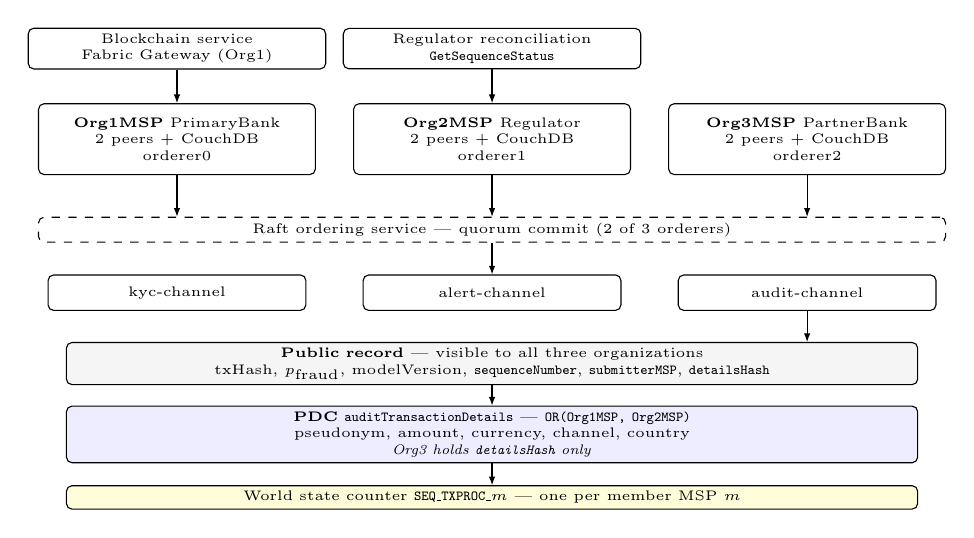
\begin{tikzpicture}[x=\columnwidth,y=1cm,font=\tiny]

% --- upstream / verifier ---------------------------------------------------
\node[draw,rounded corners=2pt,align=center,inner sep=2pt,
      text width=0.30\columnwidth] (gw) at (0.17,1.15)
  {Blockchain service\\ Fabric Gateway (Org1)};
\node[draw,rounded corners=2pt,align=center,inner sep=2pt,
      text width=0.30\columnwidth] (reg) at (0.50,1.15)
  {Regulator reconciliation\\ \texttt{GetSequenceStatus}};

% --- organisations ---------------------------------------------------------
\node[orgbox] (o1) at (0.17,0) {\textbf{Org1MSP} PrimaryBank\\ 2 peers + CouchDB\\ orderer0};
\node[orgbox] (o2) at (0.50,0) {\textbf{Org2MSP} Regulator\\ 2 peers + CouchDB\\ orderer1};
\node[orgbox] (o3) at (0.83,0) {\textbf{Org3MSP} PartnerBank\\ 2 peers + CouchDB\\ orderer2};
\draw[thinarr] (gw)  -- (o1);
\draw[thinarr] (reg) -- (o2);

% --- raft ------------------------------------------------------------------
\node[band,minimum width=0.95\columnwidth] (raft) at (0.50,-1.15)
  {Raft ordering service --- quorum commit (2 of 3 orderers)};
\draw[thinarr] (o1) -- (o1|-raft.north);
\draw[thinarr] (o2) -- (o2|-raft.north);
\draw[thinarr] (o3) -- (o3|-raft.north);

% --- channels --------------------------------------------------------------
\node[chan] (ck) at (0.17,-1.95) {kyc-channel};
\node[chan] (ca) at (0.50,-1.95) {alert-channel};
\node[chan] (cd) at (0.83,-1.95) {audit-channel};
\draw[thinarr] (raft.south) -- (ca.north);

% --- audit record split ----------------------------------------------------
\node[pubbox,text width=0.88\columnwidth] (pub) at (0.50,-2.85)
  {\textbf{Public record} --- visible to all three organizations\\
   txHash, $p_{\text{fraud}}$, modelVersion, \texttt{sequenceNumber},
   \texttt{submitterMSP}, \texttt{detailsHash}};
\node[pdcbox,text width=0.88\columnwidth] (pdc) at (0.50,-3.75)
  {\textbf{PDC} \texttt{auditTransactionDetails} ---
   \texttt{OR(Org1MSP, Org2MSP)}\\
   pseudonym, amount, currency, channel, country\\
   \emph{Org3 holds \texttt{detailsHash} only}};
\node[draw,rounded corners=2pt,fill=yellow!15,align=center,inner sep=2pt,
      text width=0.88\columnwidth] (seq) at (0.50,-4.55)
  {World state counter \texttt{SEQ\_TXPROC\_$m$} --- one per member MSP $m$};

\draw[thinarr] (cd.south) -- (cd|-pub.north);
\draw[thinarr] (pub) -- (pdc);
\draw[thinarr] (pdc) -- (seq);

\end{tikzpicture}
\caption{Three-organization consortium. Each business organization runs two
peers and hosts one node of the Raft ordering service, so no ordering node sits
outside the consortium. All
three organizations are members of all three channels; confidentiality comes
from the private data collection and pseudonymization of
Section~\ref{sec:privacy}, not from channel exclusion. The counter
\texttt{SEQ\_TXPROC\_$m$} is the mechanism of Section~\ref{sec:complete}.}
\label{fig:network}
\end{figure}

Ordering uses a Raft service of three orderer nodes, one hosted by each business
organization, rather than concentrating ordering at a single site: the operator
of a lone orderer would be a trusted third party with privileged control over
what is committed. Raft commits a log entry only once a quorum acknowledges it,
so at least two of the three organizations must participate before any block is
committed, and no single organization can unilaterally commit or suppress one.
Block validation is \texttt{ANY Writers}, as single leader Raft requires --- the
elected leader alone signs the block it cuts --- so the multi-party guarantee
rests on quorum rather than on counting signatures per block, while changes to
the ordering configuration require \texttt{MAJORITY Admins} across the
consortium. Blocks are cut on a two second batch timeout or twenty
transactions.

The ledger is partitioned into three channels, each with its own Go chaincode:
\texttt{kyc-channel} for identity records, \texttt{alert-channel} for fraud
alerts, and \texttt{audit-channel} for processing receipts, model predictions,
and report hashes. All three organizations are members of all three channels:
the regulator has a mandate to observe every channel, and the partner bank must
see fraud signal for the consortium to be useful.

\subsection{Services and transaction path}

The platform comprises nine services behind an API gateway. Eight are Go
services communicating over gRPC; the scoring service is Python. Relational
records live in PostgreSQL, enriched transactions in MongoDB, velocity windows
and cached risk tiers in Redis, with Kafka as the event backbone. Personally
identifying fields are encrypted with AES-256-GCM via a Vault transit engine.
The scoring decision is synchronous; the ledger anchor is asynchronous and
never blocks the pipeline.



\subsection{Feature extraction and domain adaptation}
\label{sec:features}

Models are trained on Elliptic, whose features are Bitcoin specific, while the
deployment target is bank wire transfers. No public labelled bank transfer
dataset of comparable scale exists, so Elliptic labels serve as a behavioral
proxy and an explicit adaptation is defined. Of the 166 raw features, the 85
with highest LightGBM importance form the canonical input, shared by every model
and by the gRPC contract. At inference on bank data, \textbf{29 of the 85
positions} are populated from structured wire transfer fields and \textbf{56 are
zero padded}, encoding Bitcoin structural quantities such as unspent output
statistics with no banking counterpart. The 29 mapped positions cover all six
behavioral indicator categories of FATF Recommendation 16 \cite{fatf2023}: value
anomaly, velocity, geographic risk, network topology, temporal pattern, and
customer profile. In institutional deployment the architecture would be
retrained on institution specific labels, replacing the Elliptic weights
entirely.

\subsection{Risk based alerting as a governance loop}

A single global threshold is inconsistent with the risk based approach FATF
Recommendation 1 requires \cite{fatf2023}. The threshold is instead a function
of the KYC risk tier $\ell$, written on the KYC channel by an authorized
compliance officer and cached in Redis from the chain. An alert is raised when

\begin{equation}
p > \tau(\ell), \quad
\tau: \{\mathrm{LOW},\mathrm{MED},\mathrm{HIGH},\mathrm{CRIT}\} \rightarrow [0,1]
\label{eq:threshold}
\end{equation}

with $\tau =$ 0.70, 0.55, 0.40, 0.25 respectively: minimizing false positives
for compliant customers, balanced, enhanced due diligence, and maximum recall.
Detector sensitivity for a given customer is therefore not a constant inside the
bank but a value governed on a multi-party ledger. When an officer raises a
customer to CRITICAL, alerting behavior changes on the next transaction with no
retraining, and the change is itself an immutable, attributed ledger record.
Threshold manipulation, a classic route to suppressing alerts, becomes visible.

% =============================================================================
\section{Provable Audit Completeness}
\label{sec:complete}
% =============================================================================

\subsection{Threat model}

We assume the bank is rational and self interested rather than externally
compromised: it will not forge endorsements or break SHA-256, but may wish a
transaction never to have existed as far as the regulator is concerned. The
regulator runs its own peer with a full replica and can obtain an independent
count of the bank's processed volume, for example from regulatory returns. The
partner bank is honest but curious: it participates in consensus and must not
learn customer level detail. The required property is therefore not merely that
anchored records are immutable, but that the anchored set is provably complete.

\subsection{Chaincode assigned sequence numbers}

The audit chaincode maintains a counter key \texttt{SEQ\_TXPROC\_}$m$ in world
state per member MSP $m$. Algorithm~\ref{alg:receipt} gives the receipt path.
Two details carry the guarantee. First, the submitting identity $m$ is read from
the transaction creator certificate through the chaincode identity API, not from
a function argument, so a submitter cannot attribute receipts to another
organization. Second, the counter increment and the receipt write occur in one
chaincode invocation and are therefore endorsed, ordered, and committed
atomically, with the counter's read version validated at commit time by Fabric's
multiversion concurrency control.

\begin{algorithm}[t]
\caption{RecordTransactionProcessed with sequence assignment}
\label{alg:receipt}
\begin{algorithmic}[1]
\STATE \textbf{input:} public metadata $R$, private details $D$ via transient map
\STATE $m \leftarrow \mathrm{MSPID}(\mathrm{creator}(\mathit{stub}))$
  \hfill \COMMENT{from certificate}
\STATE $s \leftarrow \mathrm{GetState}(\text{\texttt{SEQ\_TXPROC\_}}m) + 1$
\STATE $R.\mathit{seq} \leftarrow s$;\;
       $R.\mathit{submitterMSP} \leftarrow m$;\;
       $R.\mathit{detailsHash} \leftarrow \mathrm{SHA\text{-}256}(D)$
\STATE $\mathrm{PutState}(\text{\texttt{SEQ\_TXPROC\_}}m,\, s)$
\STATE $\mathrm{PutState}(\mathit{recordID},\, R)$
\STATE $\mathrm{PutPrivateData}(\text{\texttt{auditTransactionDetails}},
       \mathit{recordID}, D)$
\STATE \textbf{emit} \texttt{AUDIT\_RECORDED}
\end{algorithmic}
\end{algorithm}

Let $S_m$ be the latest committed sequence for organization $m$, returned by
\texttt{GetSequenceStatus}. Because the counter advances only within committed
transactions, receipts $1,\dots,S_m$ all exist; a gap cannot commit, because a
transaction skipping a value would write a counter state inconsistent with its
read version and be invalidated. Reconciliation is then the arithmetic

\begin{equation}
\Delta_m = N_m - S_m,
\label{eq:completeness}
\end{equation}

where $N_m$ is the volume organization $m$ reports independently
(Fig.~\ref{fig:proto}). Any $\Delta_m > 0$ is a provable shortfall. The bank
cannot attribute it to lost messages, because a lost message would produce a gap
and gaps cannot exist; the only consistent explanation is that the receipts were
never submitted. Backfilling is likewise detectable: a receipt anchored late
receives a current sequence number while carrying a past \texttt{processedAt}
timestamp, so skew between sequence order and timestamp order exposes
retrospective insertion.

\begin{figure}[t]
\centering
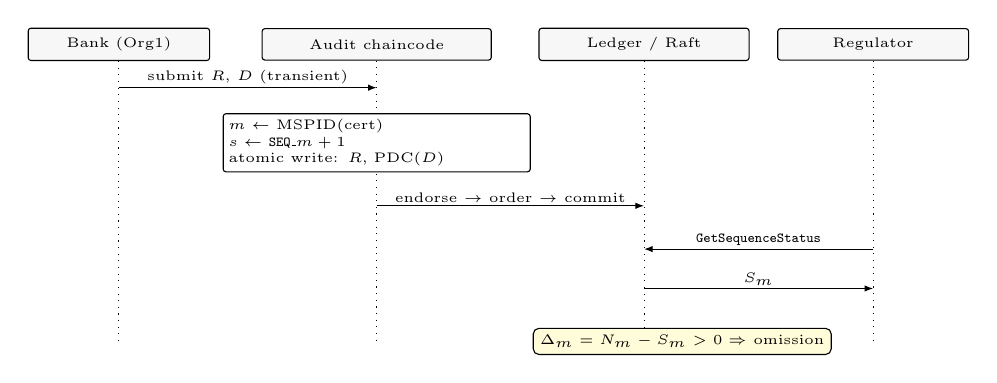
\begin{tikzpicture}[x=\columnwidth,y=1cm,font=\tiny]

\node[lane,minimum width=0.19\columnwidth] (l1) at (0.11,0) {Bank (Org1)};
\node[lane,minimum width=0.24\columnwidth] (l2) at (0.38,0) {Audit chaincode};
\node[lane,minimum width=0.22\columnwidth] (l3) at (0.66,0) {Ledger / Raft};
\node[lane,minimum width=0.20\columnwidth] (l4) at (0.90,0) {Regulator};

\foreach \n in {l1,l2,l3,l4}{\draw[dotted] (\n.south) -- ++(0,-3.55);}

% 1. submit
\draw[thinarr] (0.11,-0.55) -- node[slab,above,pos=0.5]
   {submit $R$, $D$ (transient)} (0.38,-0.55);

% 2. chaincode-internal activation
\node[draw,fill=white,rounded corners=1pt,align=left,inner sep=2pt,
      text width=0.31\columnwidth] at (0.38,-1.25)
   {$m \leftarrow$ MSPID(cert)\\
    $s \leftarrow$ \texttt{SEQ\_}$m + 1$\\
    atomic write: $R$, PDC$(D)$};

% 3. commit
\draw[thinarr] (0.38,-2.05) -- node[slab,above,pos=0.5]
   {endorse $\rightarrow$ order $\rightarrow$ commit} (0.66,-2.05);

% 4. regulator query
\draw[thinarr] (0.90,-2.60) -- node[slab,above,pos=0.5]
   {\texttt{GetSequenceStatus}} (0.66,-2.60);
\draw[thinarr] (0.66,-3.10) -- node[slab,above,pos=0.5]
   {$S_m$} (0.90,-3.10);

\node[draw,rounded corners=2pt,fill=yellow!15,inner sep=2.5pt,anchor=north]
   at (0.70,-3.60) {$\Delta_m = N_m - S_m > 0 \Rightarrow$ omission};

\end{tikzpicture}
\caption{Completeness protocol. The sequence number is assigned inside the
endorsed transaction, so the committed series is gap free. The regulator reads
$S_m$ from its own replica and compares it with the independently reported
volume $N_m$.}
\label{fig:proto}
\end{figure}

\subsection{Concurrency cost}

Every receipt from one organization reads and writes the same counter key, so
concurrent submissions conflict under MVCC. The blockchain service serializes
receipt submission with a mutex and retries validation codes 11 and 12 up to
three times. At prototype throughput this is not the binding constraint. At
production throughput the counter would need sharding, for example one counter
per day, with \eqref{eq:completeness} summed over shards. This is a real
scalability limit of the mechanism and is stated as such.

% =============================================================================
\section{Privacy Preserving Auditability}
\label{sec:privacy}
% =============================================================================

Because the audit and alert ledgers are replicated to a competing institution,
no raw identifier or business field may appear on them in plaintext; an
immutable ledger also admits no erasure, which data protection law expects.

\subsection{Keyed pseudonymization}

The blockchain service is the bank's privacy boundary. Every customer identifier
is rewritten before it leaves that boundary as
\begin{equation}
\mathit{pseudonym} = \text{\texttt{cust-}} \,\|\,
\mathrm{HMAC\text{-}SHA256}(k, \mathit{customerID}),
\label{eq:pseudonym}
\end{equation}
where $k$ is held only by the issuing bank. The transformation is one way and is
never undone; it is applied at the same boundary on both paths, to identifiers
on the way in and query arguments on the way out, so upstream services keep
using real identifiers while the ledger only ever observes pseudonyms. Because
the mapping is deterministic, the regulator can still correlate all on-chain
activity of one customer across channels, which is what an investigation
requires. Because it is keyed rather than a plain hash, a channel member holding
candidate identifiers cannot confirm any of them by recomputation, which a bare
SHA-256 would permit.

\subsection{Private data collection for receipt details}

Pseudonymization protects identity but not business fields, so the receipt is
split. The public record carries only fraud metadata --- transaction hash,
timestamp, fraud probability, risk level, alert flag, model version, sequence
number, submitting MSP --- plus the digest
$\mathit{detailsHash} = \mathrm{SHA\text{-}256}(D)$. The sensitive payload $D$
(customer pseudonym, amount, currency, channel, country) is written to the
collection \texttt{auditTransactionDetails}, whose policy is
\texttt{OR(Org1MSP.member, Org2MSP.member)}. The payload travels in Fabric's
transient field and never enters the public transaction payload, and endorsement
is restricted to collection members, so the partner bank's peer never receives
it. The anchored digest nevertheless lets the regulator prove the private data
was not altered afterwards: \texttt{GetReceiptDetails} re-hashes the retrieved
payload and returns a verification flag. The resulting split is that all three
organizations see the fraud metadata, the sequence number, and
\emph{detailsHash}, the bank and regulator additionally see the pseudonym,
amount, and corridor, and only the bank can resolve a pseudonym to a natural
person --- off-chain, and for the regulator on lawful request. Suspicious
activity reports follow the same pattern: the document is stored off-chain and only its SHA-256 digest and object
key are anchored at filing time.



% =============================================================================
\section{Evaluation}
% =============================================================================

\subsection{Dataset and protocol}

Experiments use the Elliptic Bitcoin dataset \cite{weber2019aml}: 203{,}769
transactions, 234{,}355 edges, 166 features per node, of which 94 are local and
72 aggregated from the one hop neighbourhood. Of these, 46{,}564 nodes are
labelled --- 4{,}545 illicit and 42{,}019 licit; unlabelled nodes were excluded.

The split is temporal, not random: the graph spans 49 time steps, of which
steps 1--39 form the training set and steps 40--49 the test set. A random split
leaks future information through the graph
neighbourhood and inflates reported performance; a temporal split reproduces the
deployment condition. Class imbalance was addressed with SMOTE
\cite{chawla2002smote} on the training partition only. The test partition holds
9{,}643 labelled transactions, 503 of them illicit, a prevalence of 5.22\%.

\subsection{Models and metrics}

Three tree ensembles were trained: Random Forest \cite{breiman2001randomforest}
(500 trees, depth 12, balanced class weights); XGBoost \cite{chen2016xgboost}
(500 estimators, learning rate 0.05, positive class weight 9); and LightGBM
\cite{ke2017lightgbm} (1000 leaves, learning rate 0.05, unbalanced handling).
Tree ensembles were chosen over deep alternatives because they tolerate strong
class imbalance, train in seconds rather than minutes --- which matters for the
periodic retraining a production AML programme requires --- and admit exact tree
based attribution, so every escalated alert is explainable without a surrogate
model. Every prediction carries a SHAP attribution \cite{lundberg2017shap}
serialized alongside it.

Because the positive class is rare, accuracy is near uninformative and is
reported only for comparability. We additionally report the Matthews correlation
coefficient
\begin{equation}
\mathrm{MCC} = \frac{TP \cdot TN - FP \cdot FN}
{\sqrt{(TP{+}FP)(TP{+}FN)(TN{+}FP)(TN{+}FN)}},
\label{eq:mcc}
\end{equation}
which stays meaningful under imbalance because it uses all four cells of the
confusion matrix \cite{chicco2020mcc}.

\subsection{Results}

Table~\ref{tab:models} reports performance at threshold 0.5, with the confusion
counts from which accuracy and MCC are derived.

\begin{table*}[t]
\caption{Comparative performance on the Elliptic test set (9{,}643 transactions, 503 illicit), temporal split, threshold 0.5}
\begin{center}
\setlength{\tabcolsep}{5pt}
\begin{tabular}{|l|c|c|c|c|c|c|c|c|c|c|c|}
\hline
\textbf{Model} & \textbf{Acc.\ (\%)} & \textbf{Prec.\ (\%)} & \textbf{Recall (\%)} &
\textbf{$F_1$ (\%)} & \textbf{ROC-AUC} & \textbf{MCC} & \textbf{Train (s)} &
\textbf{TN} & \textbf{FP} & \textbf{FN} & \textbf{TP}\\
\hline
LightGBM      & 96.52 & 67.08 & \textbf{65.21} & 66.13 & \textbf{0.9633} & 0.643 & \textbf{2.00} & 8979 & 161 & 175 & \textbf{328}\\
\hline
Random Forest & \textbf{97.29} & \textbf{87.12} & 56.46 & \textbf{68.52} & 0.9605 & \textbf{0.689} & 17.45 & 9098 & \textbf{42} & 219 & 284\\
\hline
XGBoost       & 96.36 & 66.52 & 60.83 & 63.55 & 0.9555 & 0.617 & 5.54 & 8986 & 154 & 197 & 306\\
\hline
\multicolumn{12}{l}{\footnotesize $^{\mathrm{a}}$Accuracy and MCC are derived from the confusion counts using \eqref{eq:mcc}. Training times measured on the same hardware.}
\end{tabular}
\end{center}
\label{tab:models}
\end{table*}

The three ensembles are close in ranking quality, with ROC-AUC between 0.956 and
0.963, but differ sharply in where they place the operating point. Random Forest
is precision oriented: it raises only 42 false positives but misses 219 of 503
illicit transactions. LightGBM is recall oriented: it recovers 328 at the cost
of 161 false positives; XGBoost falls between the two on recall while matching
neither on precision. Because the models agree closely on ranking, most of this difference is
threshold placement rather than discriminative power --- which is precisely why
the system does not hard code a threshold.

Two comparisons deserve statement. First, against the published baseline: Weber
et al.\ report illicit-class $F_1$ of 0.788 for Random Forest on all 166
features and 0.694 on the 94 local features alone \cite{weber2019aml}. Our
Random Forest reaches 0.685, essentially matching their local-feature result and
materially below their full-feature result. The likely cause is the selection of
Section~\ref{sec:features}: our 85 dimensional input retains 68 local and only
17 aggregated features, discarding most of the one hop neighbourhood signal
behind their gain. We report this openly because it bounds what the detection
layer contributes; recovering the aggregate features is straightforward future
work and is orthogonal to the accountability mechanism. Second, in absolute
terms, even the best detector leaves 175 of 503 illicit transactions unflagged.
This is the ordinary condition of AML detection, and it is exactly why the
accountability layer matters: a system missing roughly a third of illicit
activity cannot rest its credibility on detection quality alone, and must
instead demonstrate that everything it did score was recorded faithfully and
completely.

Which operating point is preferable is a compliance judgement, not a machine
learning one. A false negative costs a regulatory penalty and an open laundering
channel; a false positive costs analyst time. Under any plausible cost ratio the
recall oriented point dominates, so LightGBM was selected as the champion
detector, and it is also the cheapest to train. In deployment it is served as
the highest weighted member (0.334) of a ROC-AUC weighted ensemble over the
three tree models. The system still expresses the tradeoff per customer through
\eqref{eq:threshold}, using the same scorer at a precision oriented point for
low risk customers and a recall oriented one for critical risk customers.

\subsection{Completeness detection}
\label{sec:completenessexp}

To test whether the mechanism delivers the claimed property, we drive the audit
chaincode against Fabric's mock ledger. The bank processes $N=1000$ transactions
and suppresses a randomly chosen subset of $k$ of them, submitting no receipt at
all. This is the strongest form of the fabrication gap, because nothing is
tampered with and no record is altered. The regulator then reads $S_m$ through
\texttt{GetSequenceStatus} from its own replica, without cooperation from the
bank, and evaluates \eqref{eq:completeness}. Table~\ref{tab:completeness}
reports the outcome.

\begin{table}[htbp]
\caption{Completeness reconciliation, $N=1000$ transactions per run}
\begin{center}\footnotesize
\setlength{\tabcolsep}{4pt}
\begin{tabular}{|c|c|c|c|c|c|}
\hline
\textbf{$k$} & \textbf{$S_m$} & \textbf{$\Delta_m$} & \textbf{Detected} &
\textbf{Gap-free} & \textbf{$\mu$s/receipt}\\
\hline
0   & 1000 & 0   & ---           & yes & 38.9\\ \hline
1   & 999  & 1   & \textbf{yes}  & yes & 39.4\\ \hline
10  & 990  & 10  & \textbf{yes}  & yes & 41.9\\ \hline
100 & 900  & 100 & \textbf{yes}  & yes & 42.0\\
\hline
\multicolumn{6}{p{0.93\columnwidth}}{\footnotesize $^{\mathrm{a}}$$k$ receipts
suppressed by the bank; $S_m$ read by the regulator from its own replica;
$\Delta_m = N - S_m$. Gap-free means the committed series is exactly
$\{1,\dots,S_m\}$.}
\end{tabular}
\end{center}
\label{tab:completeness}
\end{table}

Three properties hold across every configuration. Reconciliation recovers the
suppressed count exactly, so $\Delta_m = k$ throughout, and a single omission in
one thousand transactions is as visible as a hundred. The committed series
remains exactly $\{1,\dots,S_m\}$, so suppression cannot be disguised as message
loss: a lost receipt would leave a hole, and no hole ever appears. The counter
is per organization --- 30 receipts from a second organization alongside 50 from
the first yield independent, individually gap-free series --- so one
organization's omission cannot be masked by another's volume.

We then test backfilling, the natural evasion once a shortfall is challenged.
After 100 honest receipts the bank anchors 10 more carrying \texttt{processedAt}
timestamps inside the window already covered. The series stays gap free and
$S_m$ rises to 110, so a count-only check would now balance. But every
backfilled receipt holds a sequence number above receipts bearing later
timestamps, and comparing the two orders flags exactly 10 inversions --- so the
specific insertions are identified, not merely their number.

Chaincode-side execution costs 36--46\,$\mu$s per receipt across repeated
runs, so sequence
assignment adds no meaningful cost to the write path. We state the scope of this
result plainly: it validates the completeness logic and the gap-free invariant,
not the deployed system's end-to-end commit latency or its behaviour under MVCC
contention. Those are properties of the live three-organization network.
\TODO{Report measured commit latency (p50/p95/p99) and sustained receipt
throughput per organization from \texttt{blockchain/benchmark/} once the network
run is recorded.}

\subsection{Why not an append only database}

A PostgreSQL audit log with append only triggers is simpler and faster, but its
guarantee is conditional on the honesty of whoever administers it --- in AML,
the bank under scrutiny, whose administrator can update rows, disable triggers,
and truncate write ahead logs. The single-logger constructions of Section~II-B
narrow this gap but still leave the log in the custody of the audited party. On
Fabric the regulator holds an independent replica, block commitment requires a
Raft quorum spanning three organizations, and \eqref{eq:completeness} lets the
regulator bound what it has \emph{not} been shown without issuing a challenge.
The converse holds honestly: for a single institution whose regulator trusts its
internal controls and where cross-institution sharing is not required, a
hash-chained database log suffices and blockchain is unjustified overhead.

% =============================================================================
\section{Limitations and Conclusion}
% =============================================================================

Four limitations bound these results. The models are trained on Bitcoin
features, and although the adaptation of Section~\ref{sec:features} covers all
six FATF categories, 56 of 85 positions are zero padded in bank deployment, so
the reported metrics characterize Elliptic rather than wire transfers. The
threshold ladder of \eqref{eq:threshold} is calibrated against that same score
distribution; transferring it to a bank's own features requires recalibration
rather than reuse of the published values. The sequence counter serializes an organization's receipt writes, bounding
throughput. Completeness proves count consistency, establishing that records are
missing without identifying which; binding receipts to the bank's internal
transaction numbering would pin the specific omission, at the cost of a durable
ordered anchor queue. Finally, the argument depends on $N_m$ being obtained
independently of the bank, converting the problem of trusting the audit trail
into one of trusting the volume return --- easier, but not vacuous.

This paper argued that anchoring fraud alerts on a blockchain does not make an
AML programme accountable, because the decision to raise an alert is itself the
lever a dishonest institution would pull. We presented a system in which every
scoring decision produces an immutable receipt whose series completeness is
enforced by chaincode assigned per organization sequence numbers written
atomically with each receipt, so a missing record becomes an arithmetic
shortfall computable from the regulator's own peer. Detecting omission from a
log is long studied; what is new is enforcing it inside multi-party consensus,
where the verifier is a consortium member and the ledger must withhold business
content from a competitor --- achieved through keyed pseudonymization and a
private data collection scoped to the bank and regulator. On Elliptic under a
temporal split, LightGBM achieved 65.21\% recall at 0.9633 ROC-AUC and was
selected over the higher precision Random Forest on cost asymmetry grounds.
Future work follows the limitations: sharding the counter to lift the throughput
ceiling, restoring aggregated neighbourhood features to close the detection gap,
a periodic Merkle commitment over the bank's daily transaction log, and
retraining on institution specific wire transfers.

% =============================================================================
\begin{thebibliography}{00}
\scriptsize
\setlength{\itemsep}{0pt plus 0.3pt}
\bibitem{oztas2024tm}
B. Oztas, D. Cetinkaya, F. Adedoyin, M. Budka, G. Aksu, and H. Dogan,
``Transaction monitoring in anti-money laundering: A qualitative analysis and
points of view from industry,'' \emph{Future Generation Computer Systems},
vol. 159, pp. 161--171, 2024.


\bibitem{weber2019aml}
M. Weber, G. Domeniconi, J. Chen, D. K. I. Weidele, C. Bellei, T. Robinson, and
C. E. Leiserson, ``Anti-money laundering in Bitcoin: Experimenting with graph
convolutional networks for financial forensics,'' in \emph{KDD Workshop on
Anomaly Detection in Finance}, 2019, arXiv:1908.02591.

\bibitem{elmougy2023ellipticpp}
Y. Elmougy and L. Liu, ``Demystifying fraudulent transactions and illicit nodes
in the Bitcoin network for financial forensics,'' in \emph{Proc. 29th ACM SIGKDD
Conf. Knowledge Discovery and Data Mining}, 2023.

\bibitem{pareja2020evolvegcn}
A. Pareja, G. Domeniconi, J. Chen, T. Ma, T. Suzumura, H. Kanezashi, T. Kaler,
T. B. Schardl, and C. E. Leiserson, ``EvolveGCN: Evolving graph convolutional
networks for dynamic graphs,'' in \emph{Proc. 34th AAAI Conf. Artificial
Intelligence}, 2020, pp. 5363--5370.

\bibitem{guardiola2023sealfsv2}
G. Guardiola Muzquiz and E. Soriano Salvador, ``SealFSv2: Combining
storage-based and ratcheting for tamper-evident logging,'' \emph{International
Journal of Information Security}, vol. 22, no. 2, pp. 447--466, 2023.

\bibitem{crosby2009tamperevident}
S. A. Crosby and D. S. Wallach, ``Efficient data structures for tamper-evident
logging,'' in \emph{Proc. 18th USENIX Security Symposium}, 2009, pp. 317--334.

\bibitem{kang2019fabzk}
H. Kang, T. Dai, N. Jean-Louis, S. Tao, and X. Gu, ``FabZK: Supporting
privacy-preserving, auditable smart contracts in Hyperledger Fabric,'' in
\emph{49th IEEE/IFIP Int. Conf. Dependable Systems and Networks}, 2019,
pp. 543--555.

\bibitem{khan2025baml}
A. A. Khan, A. Alsufyani, N. Alsufyani \emph{et al.}, ``BAML: A decentralized
approach to secure, privacy-preserving financial compliance for enhancing
anti-money laundering with blockchain hyperledger and federated learning,''
\emph{Peer-to-Peer Networking and Applications}, vol. 18, art. 270, 2025.

\bibitem{androulaki2018fabric}
E. Androulaki, A. Barger, V. Bortnikov \emph{et al.}, ``Hyperledger Fabric: A
distributed operating system for permissioned blockchains,'' in \emph{Proc.
Thirteenth EuroSys Conf.}, 2018, pp. 1--15.

\bibitem{breiman2001randomforest}
L. Breiman, ``Random forests,'' \emph{Machine Learning}, vol. 45, no. 1,
pp. 5--32, 2001.

\bibitem{chen2016xgboost}
T. Chen and C. Guestrin, ``XGBoost: A scalable tree boosting system,'' in
\emph{Proc. 22nd ACM SIGKDD Int. Conf. Knowledge Discovery and Data Mining},
2016, pp. 785--794.

\bibitem{ke2017lightgbm}
G. Ke, Q. Meng, T. Finley, T. Wang, W. Chen, W. Ma, Q. Ye, and T.-Y. Liu,
``LightGBM: A highly efficient gradient boosting decision tree,'' in
\emph{Advances in Neural Information Processing Systems}, vol. 30, 2017,
pp. 3146--3154.

\bibitem{chawla2002smote}
N. V. Chawla, K. W. Bowyer, L. O. Hall, and W. P. Kegelmeyer, ``SMOTE: Synthetic
minority over-sampling technique,'' \emph{Journal of Artificial Intelligence
Research}, vol. 16, pp. 321--357, 2002.

\bibitem{lundberg2017shap}
S. M. Lundberg and S.-I. Lee, ``A unified approach to interpreting model
predictions,'' in \emph{Advances in Neural Information Processing Systems},
vol. 30, 2017, pp. 4765--4774.

\bibitem{chicco2020mcc}
D. Chicco and G. Jurman, ``The advantages of the Matthews correlation
coefficient (MCC) over F1 score and accuracy in binary classification
evaluation,'' \emph{BMC Genomics}, vol. 21, art. 6, 2020.

\bibitem{fatf2023}
Financial Action Task Force, ``International standards on combating money
laundering and the financing of terrorism and proliferation: The FATF
Recommendations,'' FATF, Paris, 2023.

\end{thebibliography}

\end{document}
